\section{Metodologia}

\subsection{Viscosímetro de Stokes}

\subsection{Planagem}
    Neste experimento são utilizados dois modelos diferentes para simular o vôo de uma asa de avião. A versão mais simples consiste em um ventilados com as pás perpediculares a um aparato com uma face curva e outra reta. O aparato, doravante denominado ``asa'', tem fios atravessando verticalmente suas duas extremidades laterais ao longo do plano perpendicular às pás do ventilador. A asa fica orientada com a parte curva para cima e a parte reta para baixo. O modelo pode ser observado na \cref{asa_simples.png}.

    \begin{figure}[H]
        \centering
        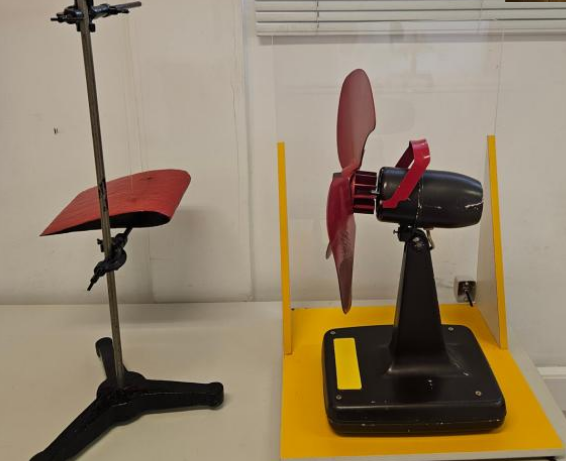
\includegraphics[width=0.35\linewidth]{fig/asa_simples.png}
        \caption{Modelo simples para estudo de planagem de uma asa de avião}
        \label{asa_simples.png}
    \end{figure}
    
    Já, a versão incluindo um tubo de pitot é construída também utilizando uma asa, porém com três furos conectados, cada um conectado a um tubo. Os três tubos são paralelos ao plano das pás do ventilador, com sentido oposto ao vetor da aceleração da gravidade. Um dos furos tem saída para a parte mais próxima das pás do ventilador; outro para a parte curva da asa; e o terceiro para a parte reta da asa. É possível observar o perfil da asa e os furos na \cref{furos.png}. Assim como no modelo simplificado, a orientação da asa é tal que a parte curva fica para cima e a parte reta para baixo. Neste modelo, a asa fica dentro de um tubo de diâmetro igual ao diâmetro do ventilador posicionado à sua frente. Ademais, a asa fica presa por um mecanismo móvel externo ao tubo que contém o ventilador e a asa. Também, os tubos conectados aos furos na asa são finos e atravessam o tubo maior que contém o ventilador e a asa. À frente do tubo que contém o ventilador e a asa, coloca-se um manômetro líquido com um tubo flexível com comprimento suficiente para conectá-lo aos tubos dos furos da asa, um de cada vez. É possível observar o modelo com tubo de pitot na \cref{asa_pitot.png}.

    \begin{figure}[H]
        \centering
        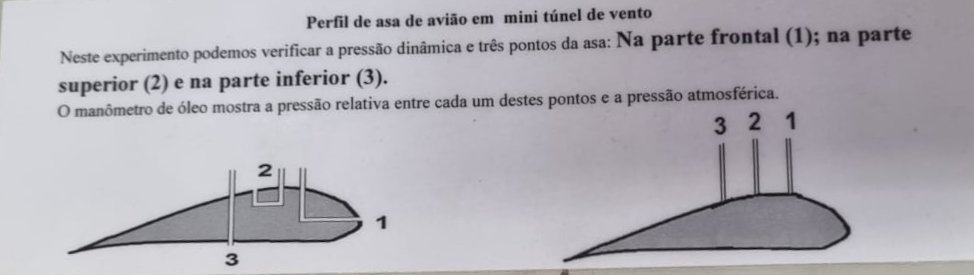
\includegraphics[width=0.35\linewidth]{fig/furos.jpeg}
        \caption{Gabarito dos furos e tubos na asa de avião do modelo com tubo de pitot} %TODO: recortar somente o gabarito
        \label{furos.png}
    \end{figure}
    \begin{figure}[H]
        \centering
        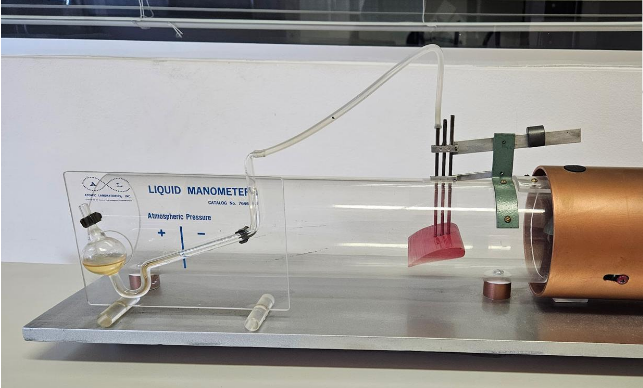
\includegraphics[width=0.35\linewidth]{fig/asa_pitot.png}
        \caption{Modelo com tubo de pitot para estudo de planagem de uma asa de avião}
        \label{asa_pitot.png}
    \end{figure}

    Para ambos os modelos, a observação é similar. No caso do modelo com tubo de pitot, primeiro deve-se conectar o tubo flexível do manômetro em um dos tubos conectados aos furos das asas. Em seguida, para ambos os modelos, deve-se ligar o ventilador e observar as variações resultantes. Em particular, para o modelo com tubo de pitot, é necessário repetir a experimentação com o manômetro conectado em cada um dos tubos.

\subsection{Tubos fechados com esferas}